% CVPR 2022 Paper Template (carried over from Lab3 submission)
% Modified for DLP Lab 5: Value-Based Reinforcement Learning.

\documentclass[10pt,twocolumn,letterpaper]{article}

\usepackage[pagenumbers]{cvpr}

\usepackage{subcaption}
\usepackage{graphicx}
\usepackage{amsmath}
\usepackage{amssymb}
\usepackage{booktabs}
\usepackage{array}
\usepackage{pgffor}
\usepackage[dvipsnames]{xcolor}
\usepackage[newfloat]{minted}
\usepackage[breakable, listings, skins, minted]{tcolorbox}
\setminted{fontsize=\footnotesize}
\renewtcblisting{minted}{%
    listing engine=minted,
    minted language=python,
    listing only,
    breakable,
    enhanced,
    minted options = {
        linenos,
        breaklines=true,
        breakbefore=.,
        numbersep=2mm
    },
    overlay={%
        \begin{tcbclipinterior}
            \fill[gray!25] (frame.south west) rectangle ([xshift=4mm]frame.north west);
        \end{tcbclipinterior}
    }
}
\usepackage{xeCJK}
\setCJKmainfont{Noto Serif CJK TC}

\usepackage[pagebackref,breaklinks,colorlinks]{hyperref}

\usepackage[capitalize]{cleveref}
\crefname{section}{Sec.}{Secs.}
\Crefname{section}{Section}{Sections}
\Crefname{table}{Table}{Tables}
\crefname{table}{Tab.}{Tabs.}

\begin{document}

\title{\LARGE Lab5 Value-Based Reinforcement Learning \\[0.5em] \large Deep Learning, NYCU}
\author{朱驛庭, 111550093}
\maketitle

%------------------------------------------------------------------------
\section{Introduction}
\label{sec:intro}

In this lab we implement \textbf{Deep Q-Network (DQN)}~\cite{mnih2015dqn} and several of its sample-efficiency enhancements -- \textbf{Double DQN (DDQN)}~\cite{hasselt2016ddqn}, \textbf{Prioritized Experience Replay (PER)}~\cite{schaul2016per}, \textbf{multi-step return}~\cite{sutton2018rl}, plus \textbf{Dueling}~\cite{wang2016dueling}, \textbf{Noisy networks}~\cite{fortunato2018noisy} and \textbf{Huber loss} -- on two environments of contrasting difficulty:
\begin{itemize}
    \item \textbf{Task 1 -- CartPole-v1}: 4-D state, 2 actions, MLP DQN. The environment converges in minutes, so we use it as a sandbox for fast iteration.
    \item \textbf{Task 2 -- ALE/Pong-v5 (vanilla DQN)}: stacked $84{\times}84{\times}4$ frames, 6 actions, CNN Q-network.
    \item \textbf{Task 3 -- ALE/Pong-v5 (enhanced DQN)}: vanilla DQN augmented with the six tricks above. The first env-step at which the agent reaches mean reward $\geq 19$ is what the spec grades.
\end{itemize}

\paragraph{Most important findings.}
\begin{enumerate}
    \item Task 1: with the right loss function (MSE in our ablation, see \cref{sec:bonus-loss}), vanilla DQN solves CartPole-v1 perfectly with mean reward $500.00$ over the 20 spec seeds.
    \item Task 2: tightening the hyper-parameters towards the original Mnih et al.\ recipe~\cite{mnih2015dqn} is enough for vanilla CNN-DQN to clear the spec threshold, hitting mean reward $19.65$.
    \item Task 3: stacking all six tricks on top of the Task 2 baseline pushes the agent across the spec threshold of mean reward $\geq 19$ at \textbf{1.5M env-steps} (snapshot mean $19.10$), earning the $15\%$ sample-efficiency bracket.
\end{enumerate}

\paragraph{Report organisation.}
\Cref{sec:implement} explains, for each spec-required item, both \emph{how the method works} and \emph{how we implemented it}, motivated by the five limitations of vanilla DQN identified in lecture.
\Cref{sec:analysis} presents the spec-evaluation screenshots, the Task 1 loss ablation, the Task 2 hyper-parameter tightening path, the Task 3 sample-efficiency comparison, and a per-technique ablation discussion.

%------------------------------------------------------------------------
\section{Implementation Details} \label{sec:implement}

We refactored the single-file template into a small \texttt{src/} package -- \texttt{src/networks.py} (\texttt{DQN}, \texttt{NoisyLinear}), \texttt{src/buffers.py} (\texttt{ReplayBuffer}, \texttt{PrioritizedReplayBuffer}), \texttt{src/preprocessor.py}, \texttt{src/agent.py} (\texttt{DQNAgent}, also home to the $n$-step deque), and \texttt{src/utils.py}. The driver \texttt{dqn.py} stays as the entry point. We deliberately renamed \texttt{AtariPreprocessor} to simply \texttt{Preprocessor} -- the same class transparently handles both the vector observation of CartPole-v1 and the $210{\times}160{\times}3$ pixel observation of Pong-v5, so the \texttt{Atari} prefix would be misleading. The other three required class names (\texttt{DQN}, \texttt{PrioritizedReplayBuffer}, \texttt{DQNAgent}) are kept as-is.

\subsection{Bellman Error for DQN} \label{sec:bellman-error}

The vanilla DQN loss in Eq.~(1) of the spec is the squared TD error
\[
    \mathcal{L}_\mathrm{DQN}(\theta) = \tfrac{1}{2}\left(r + \gamma \max_{a'} Q(s',a';\bar\theta) - Q(s,a;\theta)\right)^2,
\]
where $\bar\theta$ is the \emph{target network}, frozen for \texttt{target-update-frequency} updates and then hard-copied from the online network $\theta$. The Bellman error is computed once per gradient step inside \texttt{DQNAgent.train}; the core ten lines are:

\begin{minted}
q_values = self.q_net(states).gather(1, actions.unsqueeze(1)).squeeze(1)
with torch.no_grad():
    next_q_values = self.target_net(next_states).max(1)[0]

    # Multi-step return
    gamma_n = self.gamma ** self.n_step
    target_q_values = returns + gamma_n * (1.0 - dones) * next_q_values

td_errors = q_values - target_q_values
loss = loss_fn(td_errors, weights, self.loss_fn_type, self.huber_beta)
\end{minted}

Two points worth emphasising. First, the variable \texttt{td\_errors} is the \emph{sample} Bellman error $\delta_i = Q_\theta(s_i, a_i) - y_i$ on the sampled minibatch -- not the true Bellman residual, which would require an expectation over the transition kernel that we do not have access to. The whole DQN training procedure is essentially stochastic gradient descent on the squared sample Bellman error, with the target $y_i = r + \gamma^n \max_{a'} Q_{\bar\theta}(s', a')\cdot (1-d)$ treated as a fixed regression label thanks to \texttt{torch.no\_grad()}. Second, \texttt{returns} is already the $n$-step bootstrapped return assembled by the agent (\cref{sec:nstep}), so the same line of code handles both the 1-step and the multi-step setting via the \texttt{gamma\_n} factor. The scalar loss is then produced by our own \texttt{loss\_fn} (\cref{sec:huber-loss}), which folds in the PER importance-sampling weights. With this scaffold in place, \cref{sec:enhancements} layers six well-known enhancements on top, each motivated by a specific limitation of vanilla DQN.

\subsection{Six Enhancements over Vanilla DQN} \label{sec:enhancements}

\Cref{fig:vanilla_limit} reproduces the lecture slide that motivates Rainbow~\cite{hessel2018rainbow}: it lists five well-known limitations of vanilla DQN, and the table beneath it maps each limitation to the canonical fix. We adopt all five fixes plus a sixth one ($n$-step return) which complements them.

\begin{figure}[h]
    \centering
    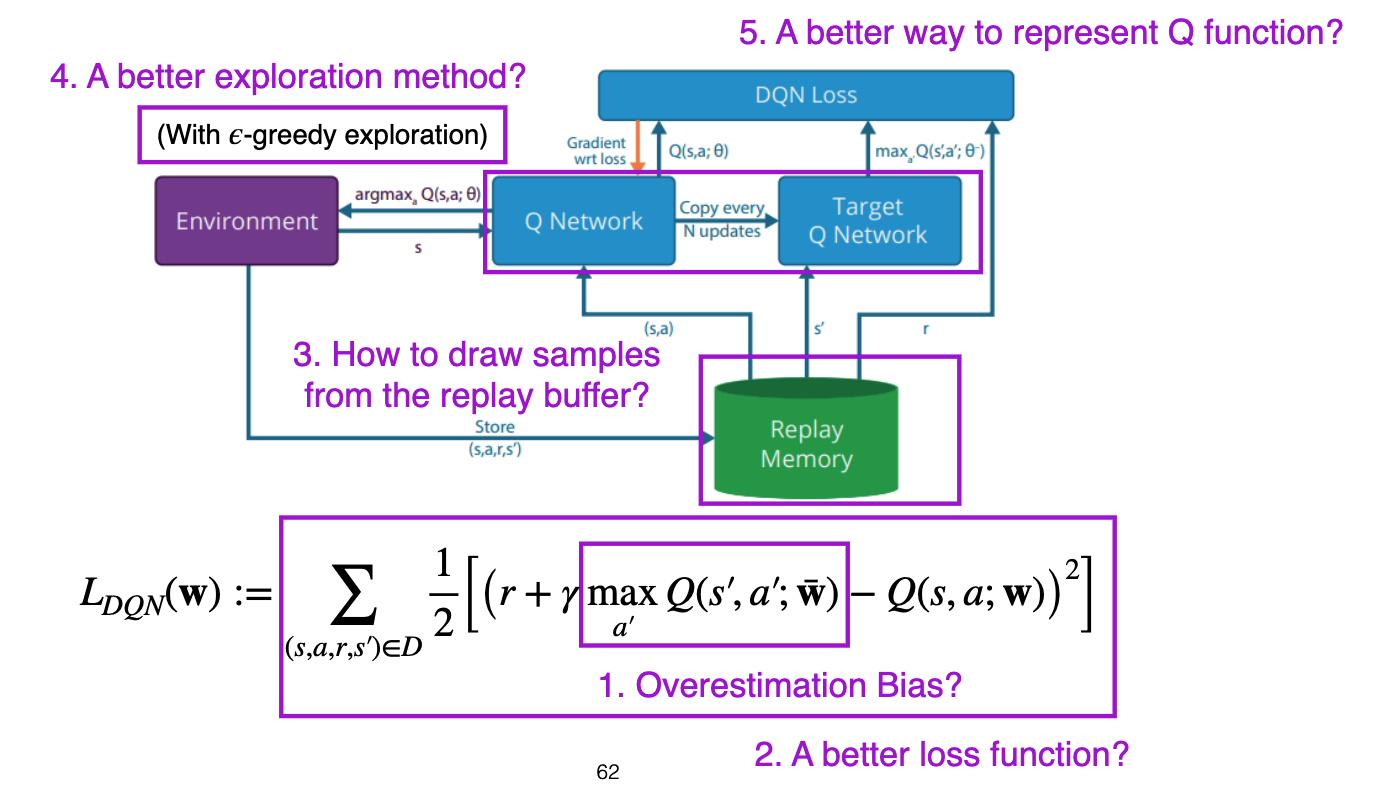
\includegraphics[width=\linewidth]{assets/pong-efficiency/vanilla-dqn-limit.png}
    \caption{The five limitations of vanilla DQN identified in the lecture slide \texttt{20260416-Value-Based-RL.pdf}. Each row of \cref{tab:tricks} names the limitation and the corresponding trick.}
    \label{fig:vanilla_limit}
\end{figure}

\begin{table}[h]
    \centering
    \footnotesize
    \begin{tabular}{p{0.50\linewidth}p{0.40\linewidth}}
        \toprule
        \textbf{Vanilla DQN limitation} & \textbf{Trick} \\ \midrule
        1. Overestimation bias from $\max_a Q$            & \textbf{Double DQN} \\
        2. Quadratic loss explodes on large TD errors     & \textbf{Huber loss} \\
        3. Uniform replay wastes informative samples      & \textbf{Prioritized Replay} \\
        4. $\varepsilon$-greedy exploration is too crude  & \textbf{Noisy networks} \\
        5. Single-stream Q-net entangles $V$ and $A$      & \textbf{Dueling networks} \\
        \midrule
        (+ slow credit assignment from 1-step bootstrap)  & \textbf{$n$-step return} \\
        \bottomrule
    \end{tabular}
    \caption{The six enhancements implemented on top of vanilla DQN in our Task 3 agent. The first five answer the lecture's five limitations; $n$-step return additionally accelerates credit assignment, as in Rainbow~\cite{hessel2018rainbow}.}
    \label{tab:tricks}
\end{table}

The next paragraphs describe each row -- both the concept and our concrete implementation.

\subsubsection{Double DQN (limitation 1)}

Vanilla DQN uses the same target network both to \emph{select} the best next action and to \emph{evaluate} that action. Because the target uses a max over noisy Q estimates, random positive errors are more likely to be selected, which creates systematic overestimation bias. DDQN~\cite{hasselt2016ddqn} fixes this by decoupling the two roles: the online network selects the next action, while the target network evaluates it. Equation~(2) of the spec becomes
\[
    a^*(s') = \arg\max_{a'} Q(s', a';\theta), \quad \mathrm{tgt} = r + \gamma\, Q(s', a^*(s');\bar\theta).
\]
The change relative to \cref{sec:bellman-error} is exactly the \texttt{next\_actions} line -- one extra forward pass through the online net replaces the $\max$ operator on the target net:

\begin{minted}
q_values = self.q_net(states).gather(1, actions.unsqueeze(1)).squeeze(1)

with torch.no_grad():
    # DDQN: use online Q-net to *select* the next action,
    # target Q-net to *evaluate* it.
    next_actions = self.q_net(next_states).argmax(dim=1, keepdim=True)
    next_q_values = self.target_net(next_states) \
        .gather(1, next_actions).squeeze(1)

    # Multi-step return
    gamma_n = self.gamma ** self.n_step
    target_q_values = returns + gamma_n * (1.0 - dones) * next_q_values

td_errors = q_values - target_q_values
loss = loss_fn(td_errors, weights, self.loss_fn_type, self.huber_beta)
\end{minted}

DDQN is enabled with \texttt{--double-dqn}; it is on for Task 3 and off for Task 1/2.

\subsubsection{Huber Loss (limitation 2)} \label{sec:huber-loss}

The vanilla DQN objective uses squared TD error. This is fine when the TD errors are small and well-behaved, but early in Atari training the targets are noisy and a few transitions can have very large $|\delta|$. Since MSE gives a gradient proportional to $|\delta|$, those outliers can dominate an entire minibatch and destabilise learning. Huber loss keeps the quadratic shape near zero but switches to a linear regime for large errors:
\[
    \mathcal{L}_\mathrm{Huber}(\delta) = \begin{cases}
        \tfrac{1}{2}\delta^2 / \beta & \text{if } |\delta| \leq \beta \\
        |\delta| - \tfrac{\beta}{2} & \text{otherwise.}
    \end{cases}
\]
We write the per-sample loss explicitly rather than calling \texttt{torch.nn.functional.huber\_loss}, because the same function also needs to fold in the PER importance-sampling weights and support both MSE and Huber through one switch:

\begin{minted}
def loss_fn(td_errors, weights, kind, beta=1.0):
    if kind == "mse":
        return (weights * td_errors.pow(2)).mean()
    if kind == "huber":
        abs_e = td_errors.abs()
        per_sample = torch.where(
            abs_e < beta,
            0.5 * td_errors.pow(2) / beta,
            abs_e - 0.5 * beta,
        )
        return (weights * per_sample).mean()
    raise ValueError(f"Invalid loss type: {kind!r}")
\end{minted}

We use Huber ($\beta = 1$) for Task 3 (Atari, noisy targets) and MSE for Task 1 (CartPole, smooth and deterministic) -- see \cref{sec:bonus-loss} for the controlled CartPole ablation that motivated this split.

\subsubsection{Prioritized Experience Replay (limitation 3)}

Uniform replay samples every stored transition with equal probability. This wastes many gradient steps on redundant or already-solved frames, while rare high-error transitions -- for example the first successful ball return in Pong -- may be replayed too infrequently. PER~\cite{schaul2016per} biases sampling toward transitions with large TD error by using
\[
    P(i) = \frac{p_i^\alpha}{\sum_j p_j^\alpha}, \qquad p_i = |\delta_i| + \epsilon.
\]
Because this changes the sampling distribution, we multiply each per-sample loss by the importance-sampling weight $w_i = (N \cdot P(i))^{-\beta} / \max_j w_j$ and anneal $\beta$ from $0.4$ to $1.0$. Our implementation is the simple proportional variant: a flat \texttt{np.float32} priority array plus \texttt{np.random.choice}. It is $O(N)$ per sampling call rather than sum-tree $O(\log N)$, but sampling was not the bottleneck compared with CNN forward/backward, and the simpler code was easier to verify.

\begin{minted}
class PrioritizedReplayBuffer:
    """Proportional Prioritized Experience Replay (Schaul et al., 2016)."""

    def __init__(self, capacity, alpha=0.6, beta=0.4,
                 beta_increment=2.5e-6, eps=1e-6):
        self.capacity = capacity
        self.buffer: list[Transition] = []
        self.pos = 0
        self.priorities = np.zeros((capacity,), dtype=np.float32)
        self.alpha, self.beta = alpha, beta
        self.beta_increment, self.eps = beta_increment, eps

    def add(self, transition, error=None):
        # New transitions get the max priority seen so far,
        # so they are guaranteed to be sampled at least once.
        if error is None:
            p = self.priorities.max() if len(self.buffer) > 0 else 1.0
        else:
            p = (abs(error) + self.eps) ** self.alpha
        if len(self.buffer) < self.capacity:
            self.buffer.append(transition)
        else:
            self.buffer[self.pos] = transition
        self.priorities[self.pos] = p
        self.pos = (self.pos + 1) % self.capacity

    def sample(self, batch_size):
        N = len(self.buffer)
        probs = self.priorities[:N] / self.priorities[:N].sum()
        indices = np.random.choice(N, batch_size, p=probs)
        weights = (N * probs[indices]) ** (-self.beta)
        weights /= weights.max()                       # normalise
        self.beta = min(1.0, self.beta + self.beta_increment)
        batch = [self.buffer[i] for i in indices]
        states, actions, rewards, next_states, dones = zip(*batch)
        return states, actions, rewards, next_states, dones, indices, weights

    def update_priorities(self, indices, errors):
        for idx, err in zip(indices, errors):
            self.priorities[idx] = (abs(err) + self.eps) ** self.alpha
\end{minted}

The TD-error magnitudes returned by the agent are fed back via \texttt{update\_priorities} after every gradient step. We use $\alpha = 0.6$, $\beta_0 = 0.4$ with \texttt{beta-increment} $= 2.5 \cdot 10^{-6}$ (so $\beta$ reaches $1$ around $240$k updates), and $\epsilon = 10^{-6}$ throughout Task 3.

\subsubsection{Noisy Networks (limitation 4)}

Vanilla DQN explores via $\varepsilon$-greedy: with probability $\varepsilon$ it ignores the Q-values and picks a uniformly random action. This is simple, but the randomness is state-independent and locally unstable -- in Pong, for example, the paddle may jitter up and down on consecutive frames instead of committing to a useful multi-step movement. NoisyNet~\cite{fortunato2018noisy} replaces this action-space randomness with \emph{parameter-space} noise: the policy is still stochastic, but the randomness comes from perturbing the Q-network itself, so action choices remain more coherent and state-dependent.

Concretely, \texttt{NoisyLinear} replaces the parameters $(W, b)$ of \texttt{nn.Linear} with
\[
    W = W_\mu + W_\sigma \odot \varepsilon^W, \qquad b = b_\mu + b_\sigma \odot \varepsilon^b,
\]
where $\varepsilon$ is factorised Gaussian noise and $W_\sigma, b_\sigma$ are learned noise scales. Thus the network can automatically reduce noise in well-learned regions and keep it where exploration is still useful. In our implementation, enabling \texttt{--noisy-net} replaces the final FC layers with \texttt{NoisyLinear} and sets \texttt{epsilon\_start = epsilon\_min = 0}, because exploration is now handled by the network rather than by random action selection.

\begin{minted}
class NoisyLinear(nn.Module):
    def __init__(self, in_features, out_features, sigma_init=0.5):
        super().__init__()
        self.in_features = in_features
        self.out_features = out_features
        self.weight_mu = nn.Parameter(torch.empty(out_features, in_features))
        self.weight_sigma = nn.Parameter(torch.empty(out_features, in_features))
        self.bias_mu = nn.Parameter(torch.empty(out_features))
        self.bias_sigma = nn.Parameter(torch.empty(out_features))
        self.register_buffer("weight_epsilon", torch.empty(out_features, in_features))
        self.register_buffer("bias_epsilon", torch.empty(out_features))
        self.sigma_init = sigma_init
        self.reset_parameters()
        self.reset_noise()

    def reset_parameters(self):
        mu_range = 1.0 / math.sqrt(self.in_features)
        self.weight_mu.data.uniform_(-mu_range, mu_range)
        self.bias_mu.data.uniform_(-mu_range, mu_range)
        self.weight_sigma.data.fill_(self.sigma_init / math.sqrt(self.in_features))
        self.bias_sigma.data.fill_(self.sigma_init / math.sqrt(self.out_features))

    @staticmethod
    def _scale_noise(size):
        x = torch.randn(size)
        return x.sign().mul_(x.abs().sqrt_())

    def reset_noise(self):
        eps_in = self._scale_noise(self.in_features)
        eps_out = self._scale_noise(self.out_features)
        self.weight_epsilon.copy_(eps_out.outer(eps_in))
        self.bias_epsilon.copy_(eps_out)

    def forward(self, x):
        if self.training:
            weight = self.weight_mu + self.weight_sigma * self.weight_epsilon
            bias = self.bias_mu + self.bias_sigma * self.bias_epsilon
        else:
            weight, bias = self.weight_mu, self.bias_mu
        return F.linear(x, weight, bias)
\end{minted}

\subsubsection{Dueling Networks (limitation 5)}

DQN estimates a separate $Q(s,a)$ for every action, even though in many states the first-order question is simply whether the state itself is good or bad. In Pong, for example, when the ball is far from the paddle, most actions have almost the same immediate value; what matters more is the state value (are we likely to win this rally?) than the tiny action differences. Dueling networks~\cite{wang2016dueling} encode this intuition by splitting $Q(s,a)$ into a state-value stream $V(s)$ and an advantage stream $A(s,a)$: first judge the quality of the state, then judge each action's relative advantage within that state. The two streams are recombined as
\[
    Q(s,a) = V(s) + \big(A(s,a) - \tfrac{1}{|\mathcal{A}|}\sum_{a'} A(s,a')\big).
\]
The mean subtraction normalises the advantage stream and makes the decomposition identifiable: $V(s)$ captures the shared state quality, while $A(s,a)-\mathrm{mean}_{a'}A(s,a')$ captures only the relative preference among actions. In code, \texttt{--dueling-dqn} swaps the single FC head for two parallel heads (\texttt{Linear} or \texttt{NoisyLinear}, depending on \texttt{--noisy-net}) and performs the recombination in \texttt{forward}:

\begin{minted}
def _build_head(self, head_in: int, num_actions: int) -> None:
    L = self._linear_cls
    if self._mode == "cnn":
        stream = lambda out: nn.Sequential(L(head_in, 512), nn.ReLU(), L(512, out))
    else:
        stream = lambda out: L(head_in, out)

    if self.dueling:
        self.value_stream = stream(1)
        self.advantage_stream = stream(num_actions)
    else:
        self.fc = stream(num_actions)

def forward(self, x: torch.Tensor) -> torch.Tensor:
    if self._mode == "cnn":
        x = x.float() / 255.0
    features = self.features(x)
    if self.dueling:
        value = self.value_stream(features)
        advantage = self.advantage_stream(features)
        return value + (advantage - advantage.mean(dim=1, keepdim=True))
    return self.fc(features)
\end{minted}

\subsubsection{$n$-step Return} \label{sec:nstep}

The original 1-step DQN target only propagates reward back by one transition per update. This is slow in Pong because the reward is sparse: most frames have reward $0$, and the $+1/-1$ signal only appears after a rally ends. $n$-step return makes the target less myopic by accumulating several real rewards before bootstrapping from the target network. For a transition starting at time $t$, we store the composite return
\[
    R_t^{(n)} = \sum_{k=0}^{n-1} \gamma^k r_{t+k}.
\]
The Bellman target then becomes $R_t^{(n)} + \gamma^n Q_{\bar\theta}(s_{t+n}, a^*)$ instead of the usual $r_t + \gamma Q_{\bar\theta}(s_{t+1}, a^*)$. In practice, the agent keeps a short deque, emits a composite transition once it has collected $n$ steps, and flushes the remaining tail transitions at the end of an episode:

\begin{minted}
def _compute_n_step(self):
    s0, a0, _, _, _ = self.n_step_buffer[0]
    _, _, _, s_last, done_last = self.n_step_buffer[-1]
    r_n = 0.0
    s_n, done_n = s_last, done_last
    for k, (_, _, r, s_next, done) in enumerate(self.n_step_buffer):
        r_n += (self.gamma ** k) * r
        s_n, done_n = s_next, done
        if done:                       # truncate at terminal
            break
    return s0, a0, r_n, s_n, done_n

def store_transition(self, s, a, r, s_next, done):
    self.n_step_buffer.append((s, a, r, s_next, bool(done)))
    if len(self.n_step_buffer) < self.n_step:
        return                          # warm-up: not enough yet
    self.memory.add(self._compute_n_step())

def on_episode_end(self):
    # Flush the tail so the last (n-1) transitions are not lost.
    while len(self.n_step_buffer) > 0:
        self.memory.add(self._compute_n_step())
        self.n_step_buffer.popleft()
\end{minted}

This is exactly why the loss code in \cref{sec:bellman-error} uses \texttt{gamma\_n = self.gamma\,**\,self.n\_step}. The trade-off is bias--variance: larger $n$ gives faster credit assignment but noisier targets. We use $n=3$ for Task 3 as a conservative middle ground.

\subsection{W\&B Tracking}

The original template logged everything into one flat namespace, which quickly became hard to read once we started running parallel ablations. I reorganised the logs into semantic groups and explicitly bound each group to the correct x-axis with \texttt{wandb.define\_metric}. The resulting dashboard separates environment-step curves from gradient-update curves, so the spec-required plots in \cref{sec:analysis} use the intended axis without manual relabelling.

\begin{center}
\small
\setlength{\tabcolsep}{5pt}
\begin{tabular}{@{}p{0.18\linewidth}p{0.49\linewidth}p{0.23\linewidth}@{}}
\toprule
\textbf{Group} & \textbf{Representative metrics} & \textbf{x-axis} \\
\midrule
\texttt{rollout/*} & episode return, length, epsilon & \texttt{env\_step} \\
\texttt{eval/*}    & 20-seed eval reward, best reward & \texttt{env\_step} \\
\texttt{train/*}   & TD error, Q statistics, loss, PER $\beta$ & \texttt{update\_step} \\
\texttt{global/*}  & raw counters for env/update steps & -- \\
\bottomrule
\end{tabular}
\end{center}

%------------------------------------------------------------------------
\section{Analysis and Discussions} \label{sec:analysis}

All numbers reported below follow the spec evaluation protocol (\S 4.2.2): 20 episodes with seeds $0,1,\ldots,19$, reporting the mean and standard deviation of undiscounted episode return. The terminal screenshots are collected at the end of the report in \cref{sec:eval-screenshots}; the main analysis keeps only the compact numerical summary and the training curves.

\subsection{Spec Evaluation Summary}

Task 1 reaches the CartPole cap exactly (mean $500.00 \pm 0.00$), earning the full $15/15$. Task 2 reaches mean Pong reward $19.65 \pm 1.46$, above the full-credit threshold. For Task 3, \cref{tab:task3_snapshots} shows that the $1.5$M snapshot is the first checkpoint above mean reward $19$, which is the submitted $15/20$ sample-efficiency bracket; the \texttt{best} checkpoint is numerically identical to that snapshot in our eval.

\begin{table}[h]
    \centering
    \footnotesize
    \setlength{\tabcolsep}{4pt}
    \begin{tabular}{@{}lccc@{}}
        \toprule
        \textbf{Snapshot} & \textbf{Mean} & \textbf{$\geq 19$?} & \textbf{Bracket} \\ \midrule
        $0.6$M           & $17.10$       & no                  & --                  \\
        $1.0$M           & $17.45$       & no                  & --                  \\
        $1.5$M           & $\mathbf{19.10}$ & \textbf{yes}     & \textbf{15/20}      \\
        $2.0$M           & $18.25$       & no                  & --                  \\
        $2.5$M           & $18.60$       & no                  & --                  \\
        \texttt{best}     & $19.10$       & yes                 & --                  \\
        \bottomrule
    \end{tabular}
    \caption{Spec evaluation of every Task 3 sample-efficiency snapshot. The earliest snapshot crossing mean reward $\geq 19$ is the $1.5$M one, which earns the $15\%$ bracket on the spec grading table. The \texttt{best} checkpoint is the $1.5$M snapshot.}
    \label{tab:task3_snapshots}
\end{table}

\subsection{Task 1: CartPole Loss Ablation} \label{sec:bonus-loss}

CartPole trains in ${\sim}10$\,min, so it is the right environment to study \emph{which loss} fits a small low-noise problem before moving to Pong. With every other hyper-parameter pinned to the baseline of \cref{tab:cartpole_baseline}, we ablate four settings: MSE and Huber with $\beta \in \{1.0,\,2.5,\,5.0\}$. \Cref{fig:task1_train} is also the Task 1 training curve required by the spec, with the $x$-axis set to \texttt{global/env\_step}.

\begin{table}[h]
    \centering
    \footnotesize
    \begin{tabular}{ll}
        \toprule
        \textbf{Hyper-parameter}      & \textbf{Value} \\ \midrule
        Episodes (cap)                & $1500$ \\
        Batch size                    & $64$ \\
        Learning rate                 & $1{\times}10^{-4}$ \\
        Replay buffer                 & uniform, $100\,000$ \\
        Replay start                  & $5\,000$ \\
        Target update freq.           & $1\,000$ env-steps \\
        $\varepsilon$ schedule        & exp.\ $1.0 \rightarrow 0.05$ ($\lambda{=}0.99995$) \\
        Discount $\gamma$             & $0.99$ \\
        Eval                          & every 10 episodes, 20 seeds \\
        Early stop                    & mean reward $\geq 480$ for 3 evals \\
        Seed                          & $42$ \\
        \bottomrule
    \end{tabular}
    \caption{CartPole-v1 baseline shared across the loss ablation; only \texttt{loss-fn-type} and \texttt{huber-beta} are swept.}
    \label{tab:cartpole_baseline}
\end{table}

\begin{figure}[h]
    \centering
    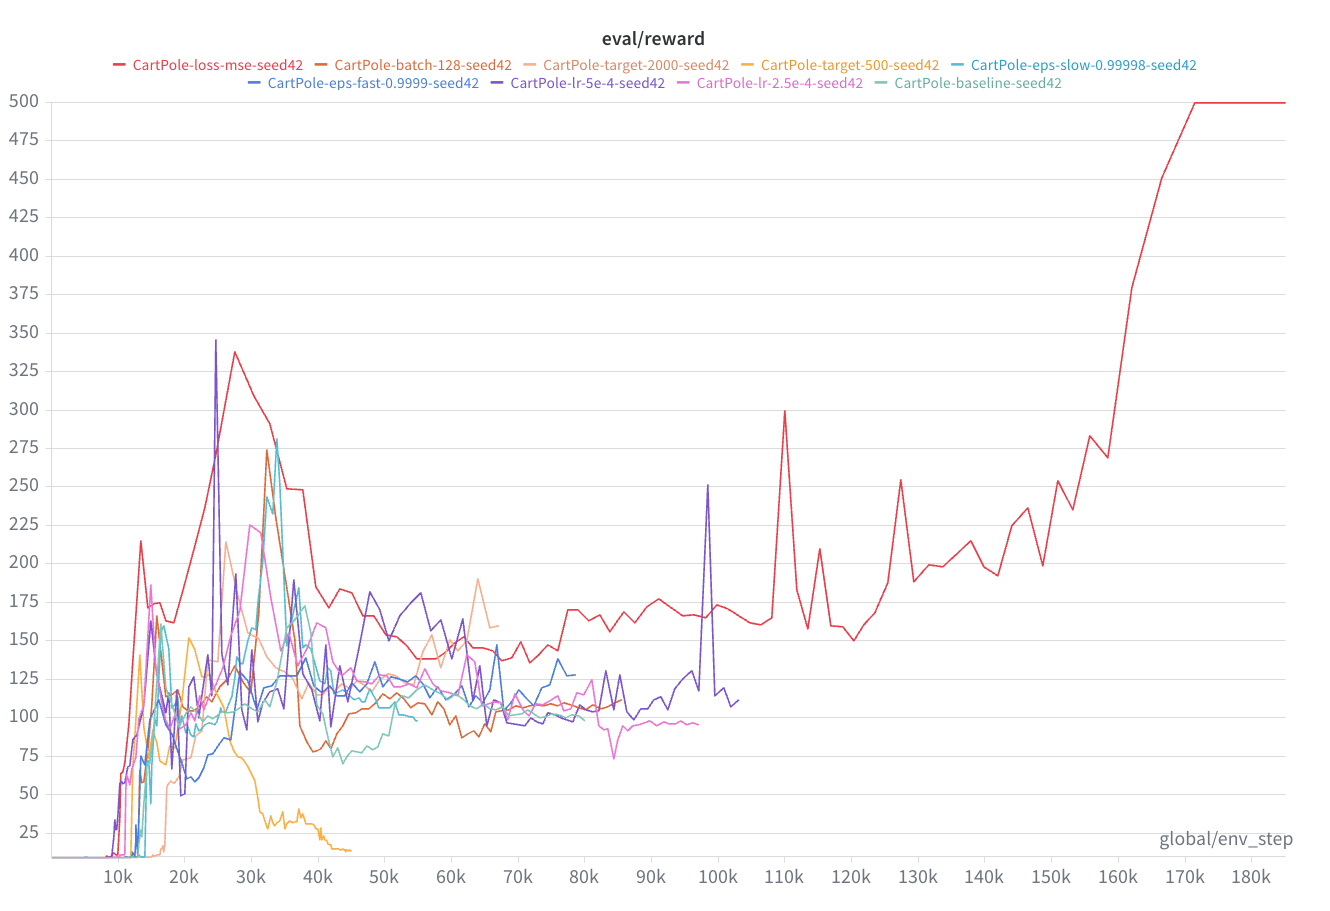
\includegraphics[width=\linewidth]{assets/cartpole-ablation/eval_reward.png}
    \caption{\textbf{Task 1} -- \texttt{eval/reward} vs.\ environment step for the four CartPole-v1 loss settings. The submitted run (\texttt{loss-mse / seed42}, blue) is the only one that reaches and stays at the maximum reward of $500$.}
    \label{fig:task1_train}
\end{figure}

\textbf{Finding.} MSE wins on this low-noise environment: it is the only setting whose evaluation reward consistently reaches $500$, and it does so faster than the Huber variants. Huber is useful later on Atari because it clips large TD-error outliers, but in deterministic CartPole those clipped gradients mostly slow down learning without providing much stability benefit. This is why the submitted Task 1 checkpoint uses MSE.

\subsection{Task 2: From Untuned Vanilla Pong to Mnih-Style DQN}

Our first Pong run (orange in \cref{fig:pong_three_way}) used hyper-parameters mostly inherited from CartPole: larger replay memory, target update every $10\,000$ env-steps, a slow exponential $\varepsilon$ decay, and no explicit train-frequency. It learned, but sample efficiency was poor. Tightening the setup toward the original Mnih et al.\ recipe~\cite{mnih2015dqn} gives the blue run, \texttt{mnih-standard}, which is still vanilla CNN-DQN but trains much faster and becomes the submitted Task 2 model.

\begin{table}[h]
    \centering
    \scriptsize
    \setlength{\tabcolsep}{3pt}
    \begin{tabular}{@{}>{\raggedright\arraybackslash}p{0.30\linewidth}>
                    {\raggedright\arraybackslash}p{0.28\linewidth}>
                    {\raggedright\arraybackslash}p{0.34\linewidth}@{}}
        \toprule
        \textbf{Hyper-param.}    & \textbf{Untuned} & \textbf{Mnih-style} \\ \midrule
        Memory size              & $200\,000$            & $100\,000$              \\
        Replay start             & $50\,000$             & $10\,000$               \\
        Target update freq.      & $10\,000$ env-steps   & $1\,000$ \emph{updates} \\
        Train frequency          & every env-step        & every $4$ env-steps     \\
        $\varepsilon$ schedule   & exp.\ $\lambda{=}10^{-7}$ & linear $1.0\to0.01$ over $10^{6}$ steps \\
        Loss                     & MSE                   & MSE \\
        \bottomrule
    \end{tabular}
    \caption{Task 2 hyper-parameter tightening: both columns are vanilla CNN-DQN; only the right column is the submitted Task 2 configuration.}
    \label{tab:pong_v2_diff}
\end{table}

\begin{figure}[h]
    \centering
    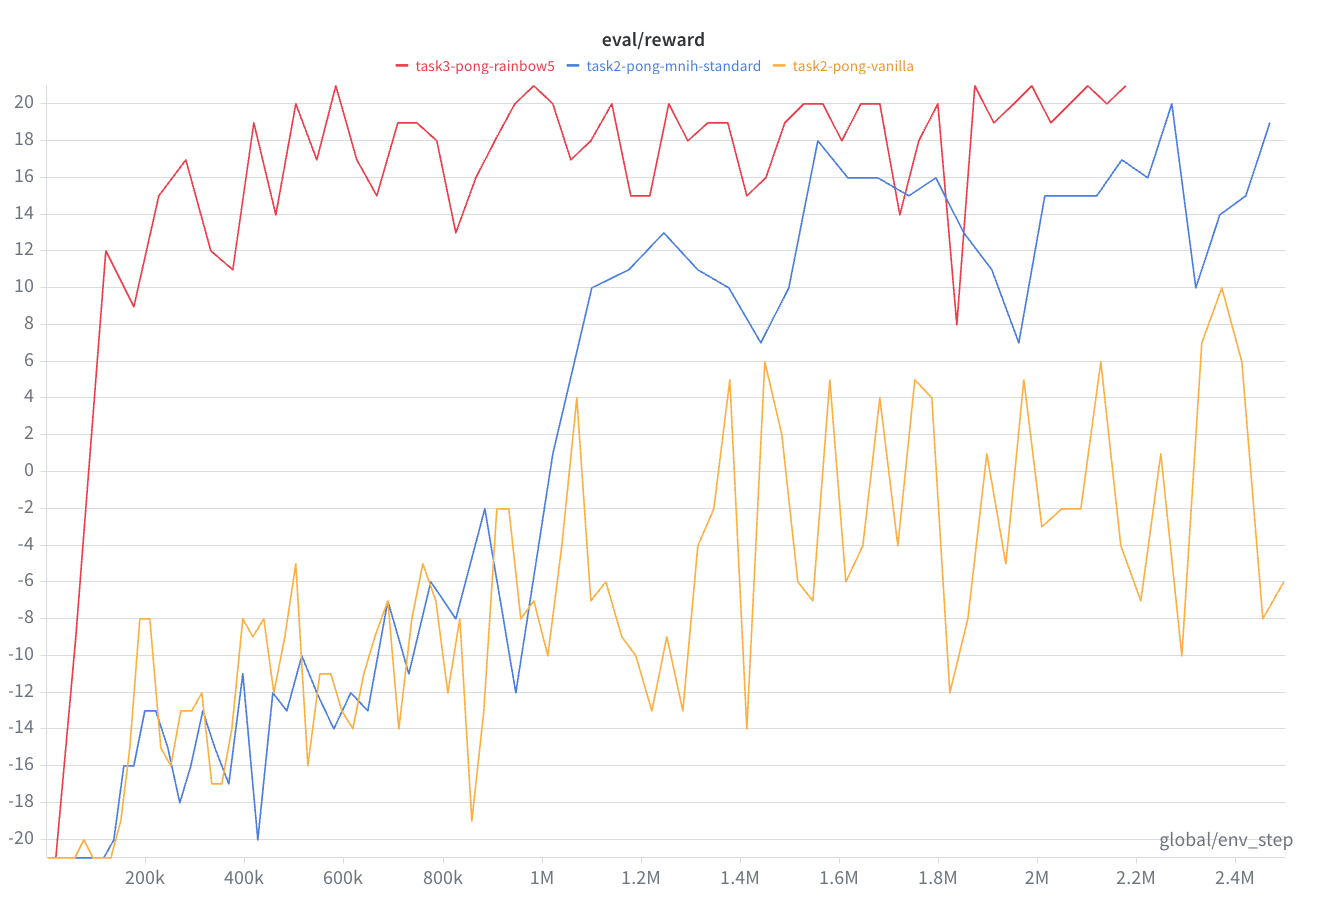
\includegraphics[width=\linewidth]{assets/pong-efficiency/eval_reward_task3_2.5M.png}
    \caption{\textbf{Pong sample efficiency} -- orange is the untuned vanilla Pong run, blue is the Mnih-style vanilla DQN submitted for Task 2, and red is the fully enhanced Task 3 agent. Hyper-parameter tightening alone greatly accelerates Task 2, while the Task 3 enhancements push the curve above the mean-reward-$19$ threshold by $1.5$M env-steps.}
    \label{fig:pong_three_way}
\end{figure}

The two Task 2 changes that matter most are: (i) targeting every $1\,000$ \emph{gradient updates} instead of every $10\,000$ env-steps, which keeps the bootstrap target close enough to the online network that Q-values can grow; and (ii) decaying $\varepsilon$ linearly to $0.01$ over $1$M env-steps, which lets policy improvement translate into rollout return instead of continuing to inject too much random action noise.

\subsection{Task 3: Enhanced DQN Sample Efficiency}

The Task 2 \texttt{mnih-standard} run and Task 3 \texttt{rainbow5} run share batch size, optimiser, learning rate, and frame stack; \cref{tab:vanilla_vs_enhanced} lists only the important differences. This makes the blue-vs-red comparison in \cref{fig:pong_three_way} a clean read on the effect of adding DDQN, PER, Huber, NoisyNet, Dueling, and $n$-step return.

\begin{table}[h]
    \centering
    \scriptsize
    \setlength{\tabcolsep}{3pt}
    \begin{tabular}{@{}p{0.28\linewidth}p{0.28\linewidth}p{0.36\linewidth}@{}}
        \toprule
        \textbf{Hyper-param.}        & \textbf{Vanilla (T2)} & \textbf{Enhanced (T3)} \\ \midrule
        Replay buffer                & uniform               & PER ($\alpha{=}0.6$, $\beta{=}0.4{\to}1$) \\
        $n$-step return              & $1$                   & $\mathbf{3}$ \\
        Bootstrap target             & vanilla DQN           & \textbf{Double DQN} \\
        Network head                 & single Q-stream       & \textbf{Dueling} V/A streams \\
        Exploration                  & $\varepsilon$-greedy linear $1{\to}0.01$ & $\varepsilon{=}0$, \textbf{NoisyNet} \\
        Loss                         & MSE                   & \textbf{Huber} ($\beta{=}1$) \\
        Memory size                  & $100\,000$            & $50\,000$ \\
        Target update freq.          & $1\,000$ updates      & $500$ updates \\
        Train freq.\,/\,per-step     & every 4 env-steps, $1$ & every 4 env-steps, $4$ \\
        \bottomrule
    \end{tabular}
    \caption{Vanilla DQN (Task 2) vs.\ enhanced DQN (Task 3) hyper-parameters. The bold rows correspond exactly to the six tricks of \cref{tab:tricks}.}
    \label{tab:vanilla_vs_enhanced}
\end{table}

The enhanced agent is dramatically more sample-efficient: at $1.5$M env-steps it has already reached spec mean reward $19.10$, while the vanilla agent at the same env-step is still around $-10$ to $0$ on \texttt{eval/reward}. The vanilla agent only catches up around the $4$--$5$M env-step range. Concretely, the enhanced agent crosses the spec threshold roughly $\mathbf{3{-}4{\times}}$ earlier in env-steps than the vanilla one.

\subsection{Per-Technique Ablation}

To isolate the effect of the three techniques originally required by the spec, we trained technique-only Pong runs on top of the same Mnih-style baseline: DDQN only, PER only, and $n$-step return only ($n=3$). We also trained an \texttt{all3} run that combines exactly these three techniques (PER + DDQN + $n$-step). This ablation intentionally does \emph{not} compare Huber, NoisyNet, or Dueling, so we do not draw conclusions about them here.

\begin{figure}[h]
    \centering
    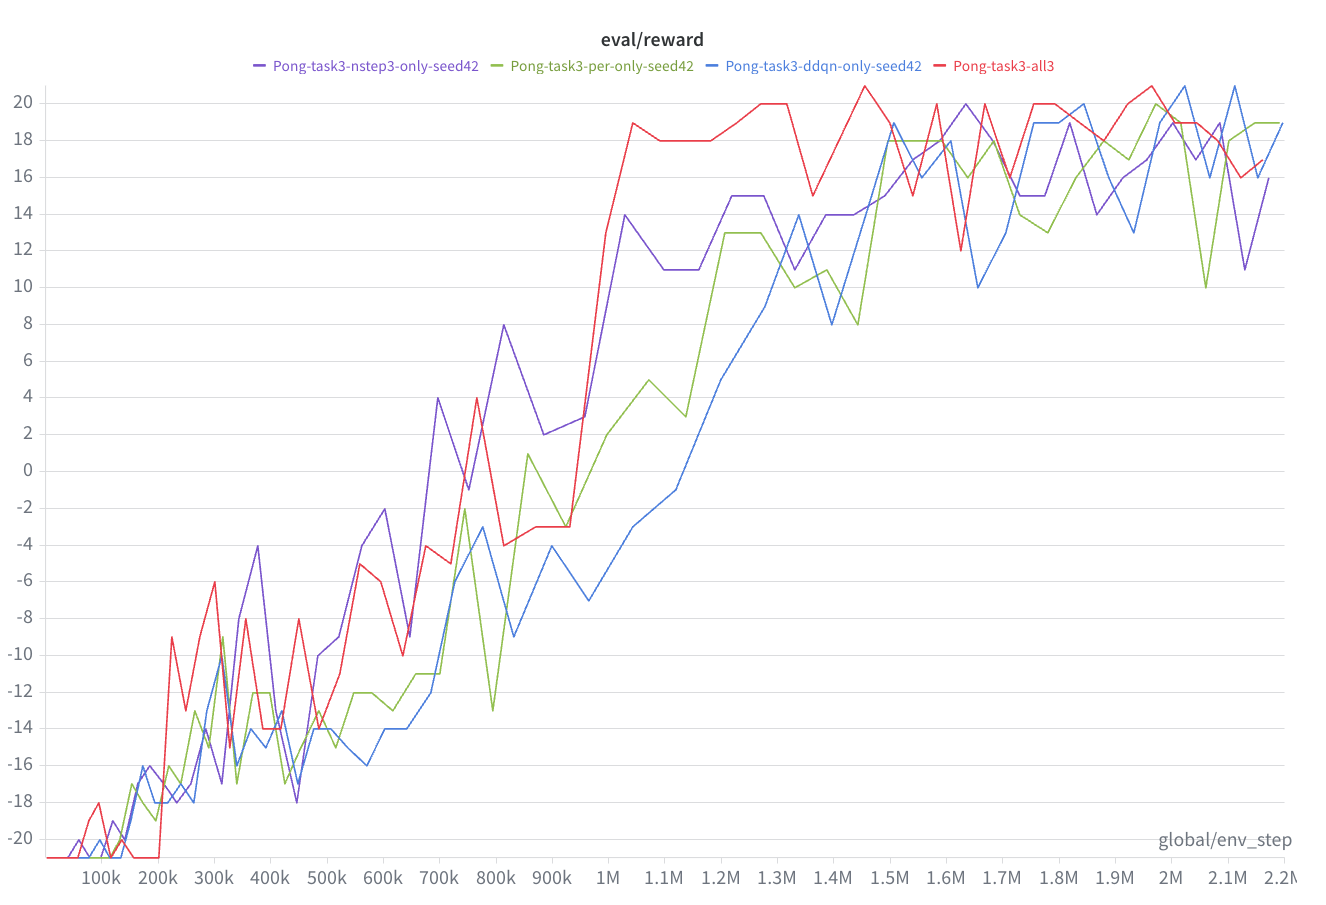
\includegraphics[width=\linewidth]{assets/pong-efficiency/per-technique-ablate.png}
    \caption{Technique-only ablation on Pong-v5. Purple, green, and blue enable only $n$-step return, PER, or DDQN respectively; red combines all three. Here ``full'' means PER+DDQN+$n$-step3, not the complete Task 3 stack with Dueling/NoisyNet/Huber.}
    \label{fig:per_technique_ablation}
\end{figure}

\paragraph{$n$-step return.} The purple curve improves earliest among the single-technique runs, reaching positive reward before the PER-only and DDQN-only curves. This matches the intuition that Pong's reward is sparse: aggregating three real rewards before bootstrapping propagates the rally outcome back faster than pure 1-step TD learning.

\paragraph{PER.} The green curve improves more gradually, but becomes competitive after roughly $1.5$M env-steps. PER helps once the replay buffer contains informative high-error transitions, because those rare ball-contact / rally-ending transitions are replayed more often than under uniform sampling.

\paragraph{DDQN.} The blue curve is the slowest early on, but catches up later and reaches high reward in the final phase. This suggests that DDQN's main benefit in this setting is not early exploration speed, but more stable bootstrap targets after the policy has started finding useful Pong behaviours.

\paragraph{Combined effect.} The red \texttt{all3} curve is best in sample efficiency: it jumps to high reward around $1.0$M env-steps and stays mostly in the $18$--$21$ range afterward. The single-technique curves eventually approach strong performance, but the combination reaches it earlier and with fewer long low-reward phases, showing that the three methods are complementary rather than redundant.

\section{Spec-Eval Screenshots} \label{sec:eval-screenshots}

For completeness, this appendix-style section records the terminal outputs used to verify the submitted checkpoints. The filenames are omitted from captions to avoid visually noisy long monospace strings; all submitted checkpoints follow the required \texttt{LAB5\_111550093\_*.pt} naming convention.

\begin{figure}[h]
    \centering
    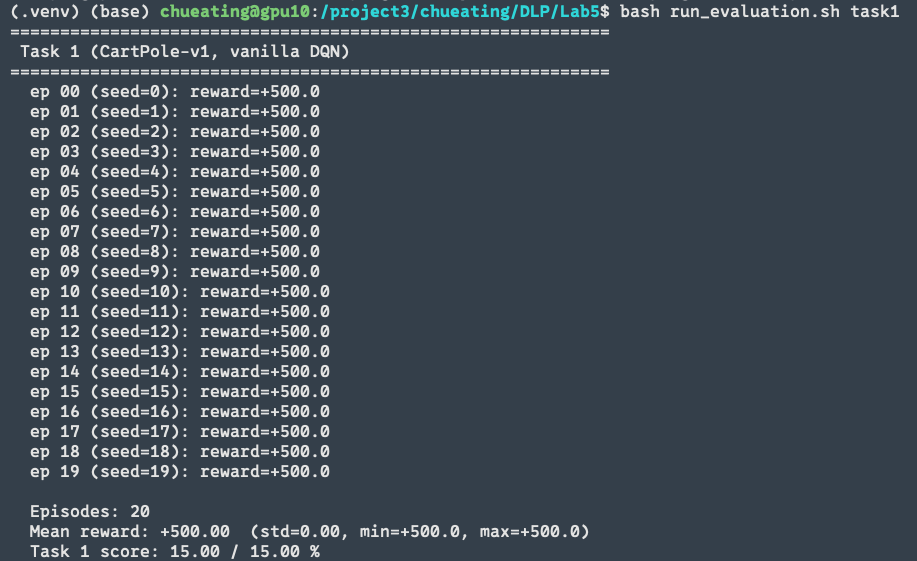
\includegraphics[width=\linewidth]{assets/screenshots/task1.png}
    \caption{Task 1 eval screenshot: mean $500.00 \pm 0.00$, score $15/15$.}
    \label{fig:task1_eval}
\end{figure}

\begin{figure}[h]
    \centering
    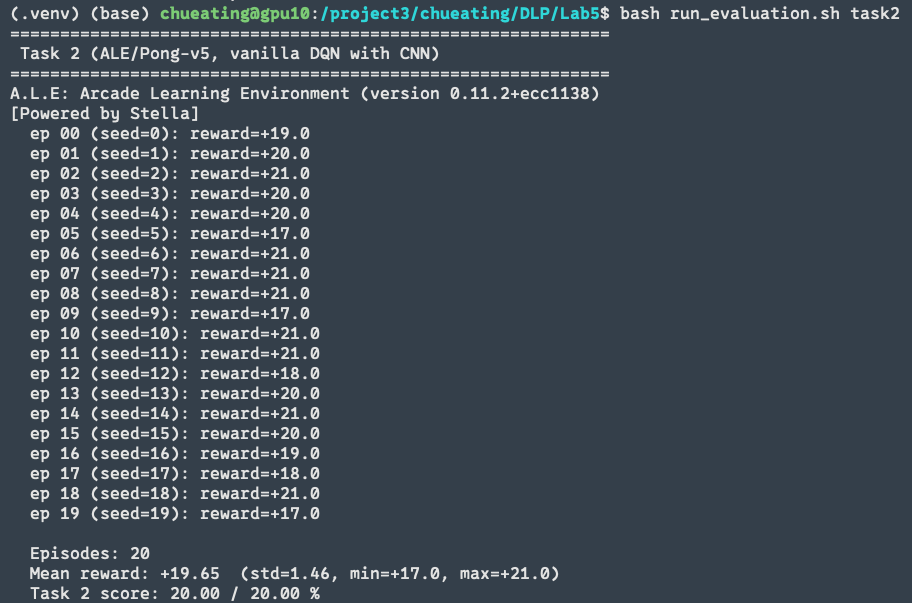
\includegraphics[width=\linewidth]{assets/screenshots/task2.png}
    \caption{Task 2 eval screenshot: mean $19.65 \pm 1.46$, score $20/20$.}
    \label{fig:task2_eval}
\end{figure}

\begin{figure}[h]
    \centering
    \begin{subfigure}{0.48\linewidth}
        \centering
        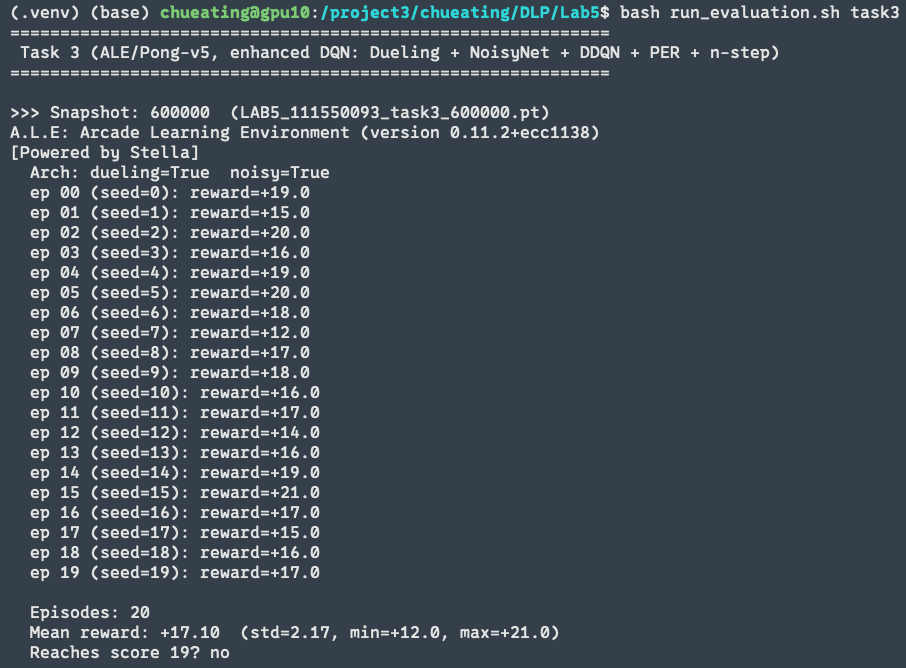
\includegraphics[width=\linewidth]{assets/screenshots/task3_600K.png}
        \caption{$0.6$M}
    \end{subfigure}
    \hfill
    \begin{subfigure}{0.48\linewidth}
        \centering
        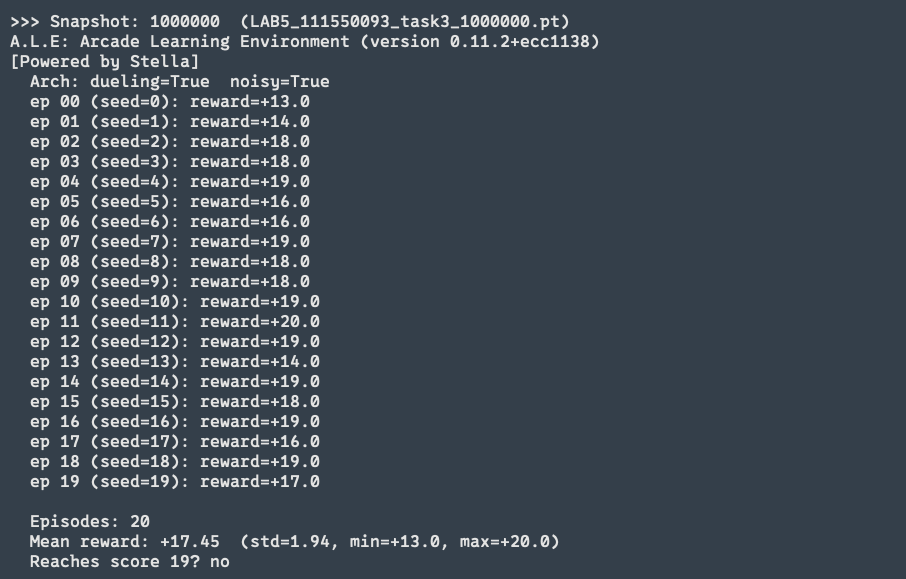
\includegraphics[width=\linewidth]{assets/screenshots/task3_1M.png}
        \caption{$1.0$M}
    \end{subfigure}

    \vspace{0.15cm}

    \begin{subfigure}{0.48\linewidth}
        \centering
        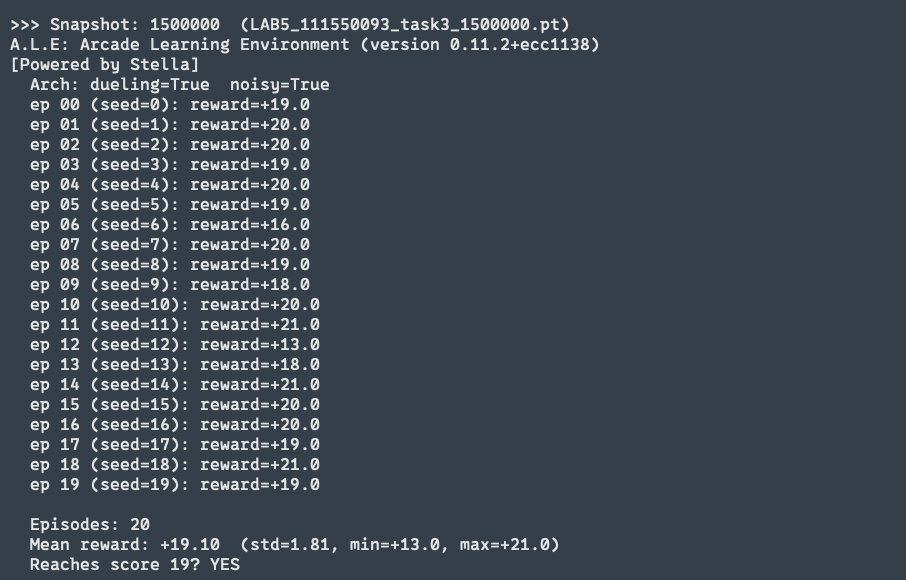
\includegraphics[width=\linewidth]{assets/screenshots/task3_1.5M.png}
        \caption{$1.5$M}
    \end{subfigure}
    \hfill
    \begin{subfigure}{0.48\linewidth}
        \centering
        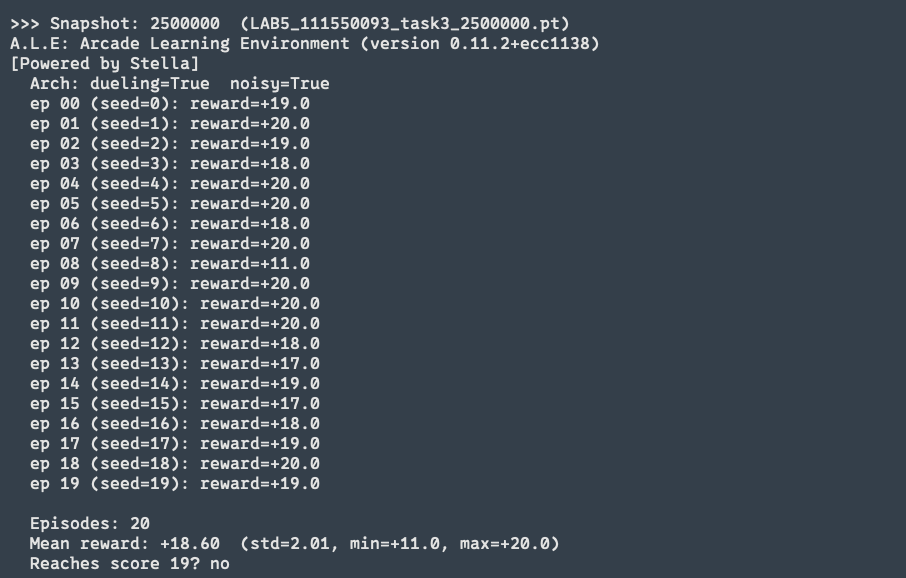
\includegraphics[width=\linewidth]{assets/screenshots/task3_2.5M.png}
        \caption{$2.5$M}
    \end{subfigure}

    \vspace{0.15cm}

    \begin{subfigure}{0.48\linewidth}
        \centering
        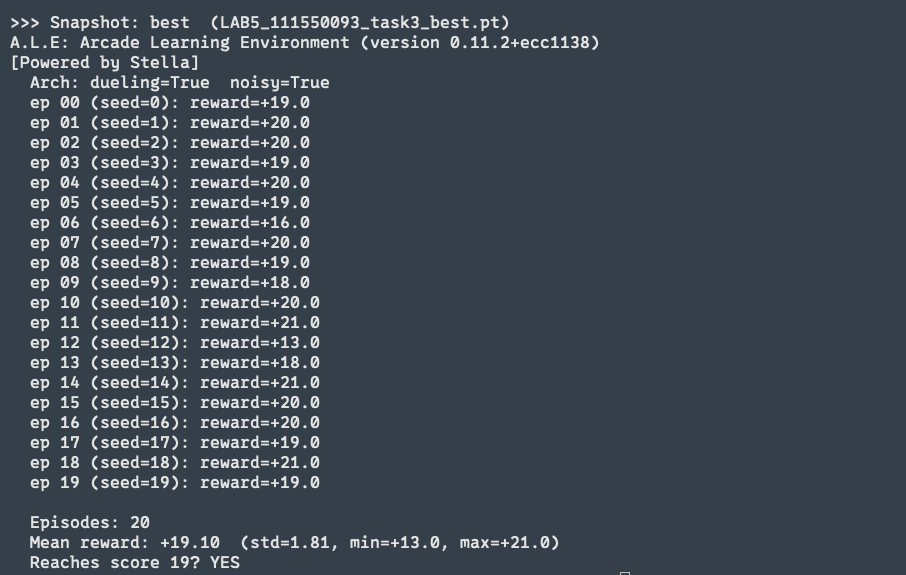
\includegraphics[width=\linewidth]{assets/screenshots/task3_best.png}
        \caption{best}
    \end{subfigure}
    \caption{Task 3 eval screenshots for sample-efficiency snapshots and best checkpoint.}
    \label{fig:task3_screenshots}
\end{figure}

%%%%%%%%% REFERENCES
{\small
    \bibliographystyle{ieee_fullname}
    \bibliography{egbib}
}

\end{document}
